\begin{figure}[H]
    \centering
     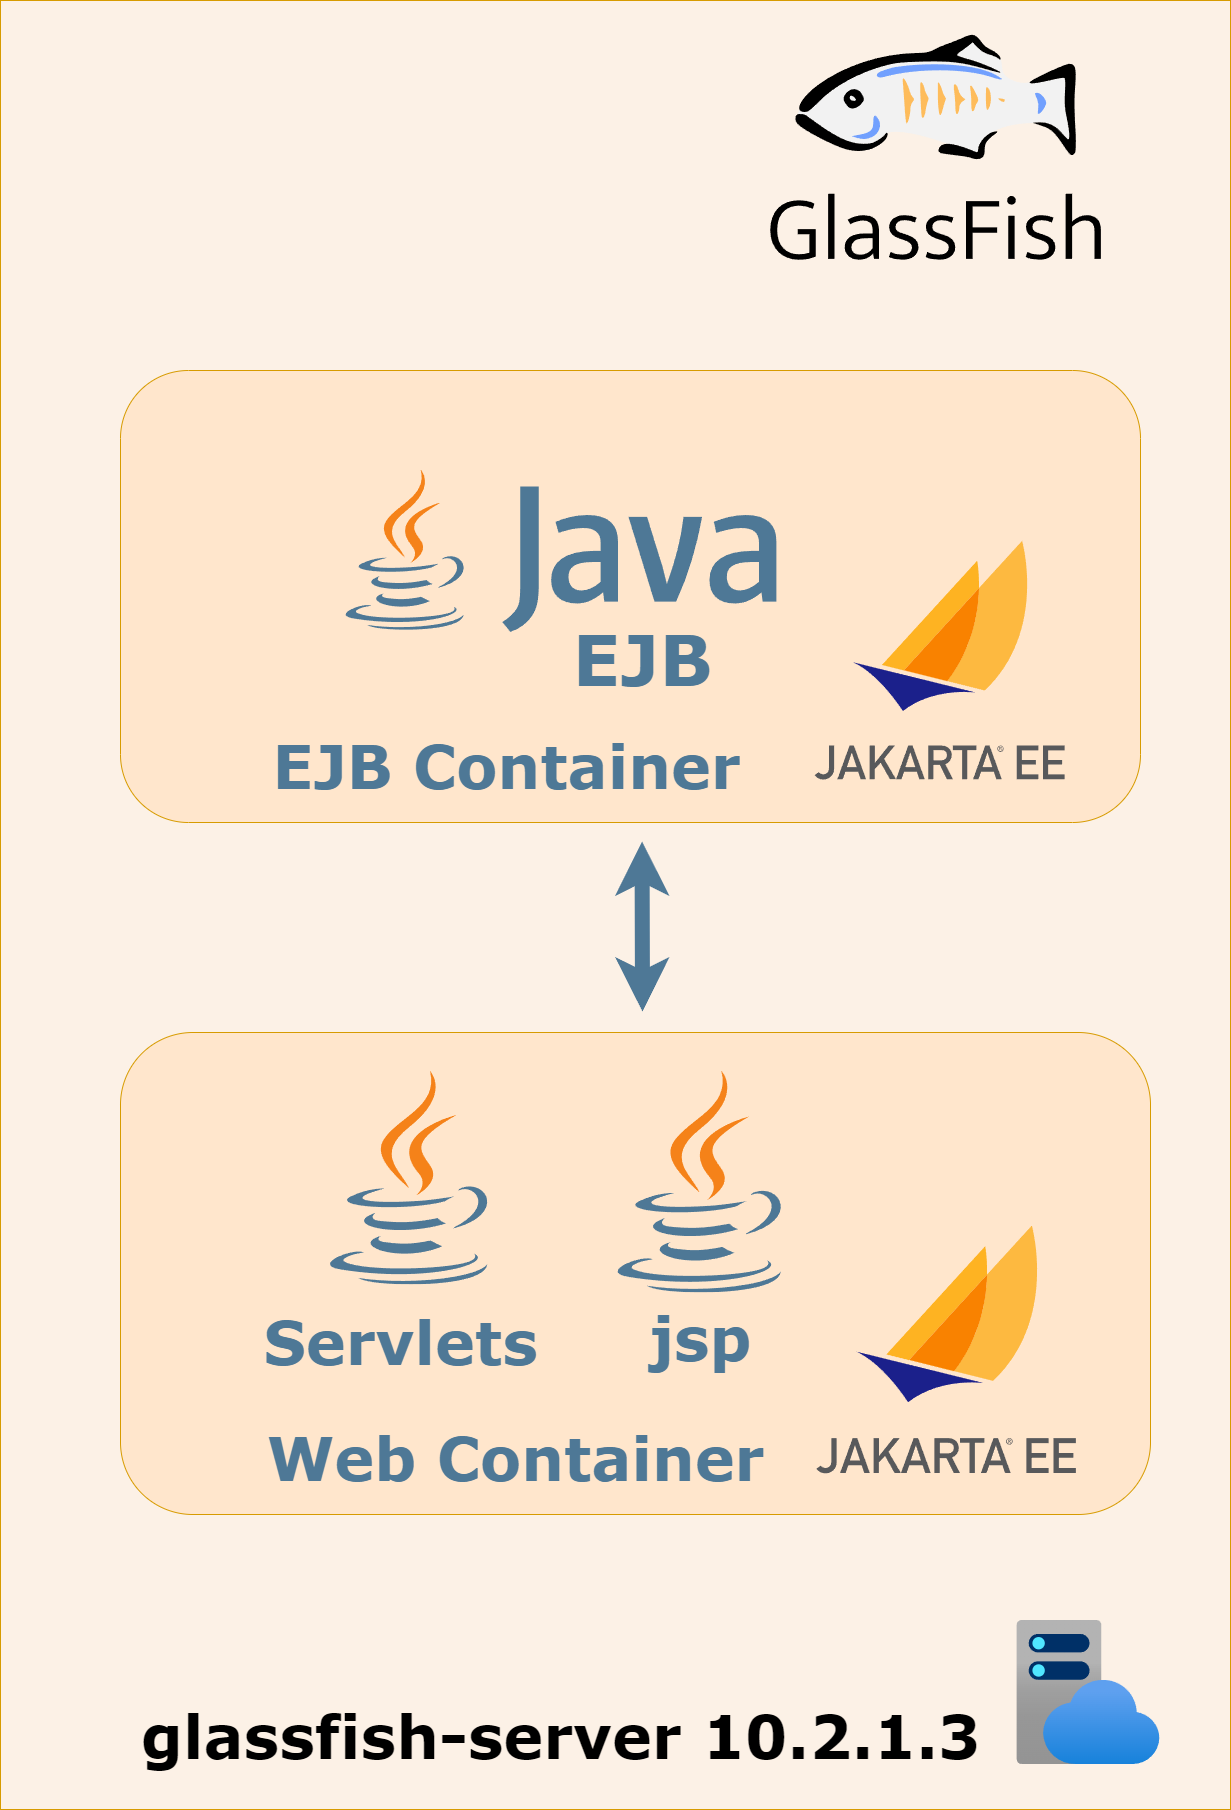
\includegraphics[width=0.45\textwidth]{img/system_architecture/glassfish-server.png}
    \caption{\label{fig:glassfish-server} Glassfish-Server Schema.}
\end{figure}

In our project we have implemented the web-app functionality through the Java EE application server known as Glasshfish. This part of the project was divided into three sub-projects in order to separate the business logic from the others application components:
\begin{itemize}
    \item \textbf{web project}: It contains servlets and Java server Pages (JSP). It is responsible for receiving requests and perform calls to EJBs in order to build the requested resources through JSP technology
    \item \textbf{ejb-interfaces}: It contains the interfaces for the calls to EJBs from Sevlets, the structure of all the DTOs and enumerated types
    \item \textbf{ejb}: It contains the implementation of all EJBs and DAOs. EJB are needed to implement all the business logic instead, DAOs, provide an interface between the application and the application's database.
\end{itemize}